\chapter{Onderzoeksopzet}
Voor dit onderzoek wordt er gebruik gemaakt van \textit{Wat is Onderzoek} \Parencite{Verhoeven}.
Dit hoofdstuk omvangt het eerste deel het ontwerpen van het onderzoek.\\

\begin{graphic}
	\vspace{0.2cm}
	\captionsetup{type=figure}
	\caption{Deel 1 Verhoeven ontwerpen}
	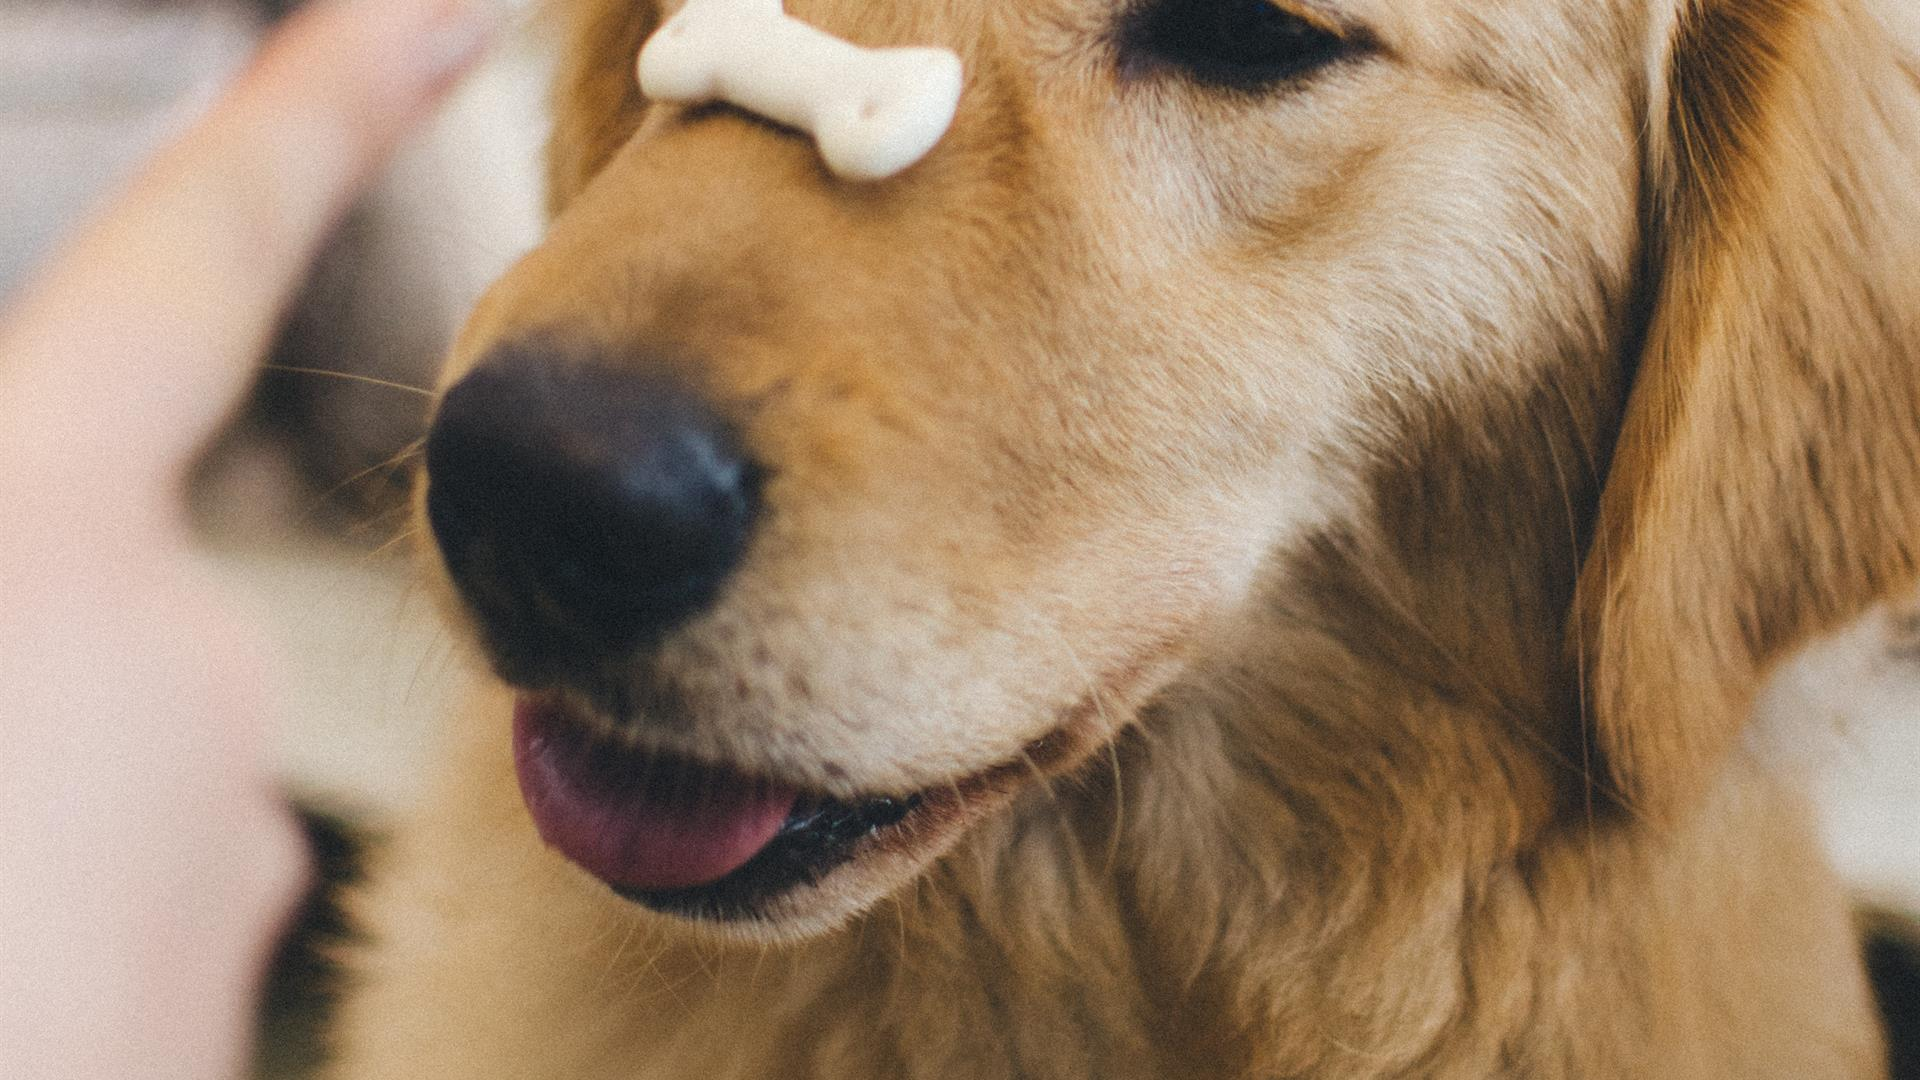
\includegraphics[scale=0.2]{img/Placeholder.jpg}
	\label{fig:Deel1Verhoeven}
	\vspace{0.2cm}
\end{graphic}

\whitespace
Eerst worden de onderzoeksvragen behandeld en daar de onderzoeksmethoden die gebruikt worden bij zet onderzoeksvragen.
\section{Doelstelling}
\label{sec:Doelstelling}
Om het proof of concept te realiseren moet er eerst bekend zijn wat er gemaakt moet worden en voor wie.
Hierom moet er een lijst aan geprioriteerde requirements komen voor 22 november 2023 voor het \qw{het CMS voor iedereen} project.
Deze lijst moet worden samengesteld in samenwerking met de stakeholders. Hierom is de volgende hoofdvraag opgesteld:

\whitespace
\begin{center}
    \textit{\MainQuestion}
\end{center}

\section{Onderzoeksvragen}
Text text text\\
\textbf{Hoofdvraag:} \textit{\MainQuestion} \\

Text text text\\

\textbf{Deelvraag 1:} \textit{\SubquestionOne}\\

\textbf{Deelvraag 2:} \textit{\SubquestionTwo} \\

\textbf{Deelvraag 3:} \textit{\SubquestionThree} \\
text\\ 
\textbf{Deelvraag 4:} \textit{\SubquestionFour} \\

\textbf{Deelvraag 5:} \textit{\SubquestionFive} \\

\section{Onderzoeksmethoden}
onderzoeksmethoden\\
\textbf{Deelvraag 1:} \textit{\SubquestionOne}\\

\textbf{Deelvraag 2:} \textit{\SubquestionTwo} \\

\textbf{Deelvraag 3:} \textit{\SubquestionThree} \\
text\\ 
\textbf{Deelvraag 4:} \textit{\SubquestionFour} \\

\textbf{Deelvraag 5:} \textit{\SubquestionFive} \\

